
%(BEGIN_QUESTION)
% Copyright 2010, Tony R. Kuphaldt, released under the Creative Commons Attribution License (v 1.0)
% This means you may do almost anything with this work of mine, so long as you give me proper credit

A pneumatically-operated cylinder used to actuate the ash grate on a coal-fired furnace refuses to actuate when the operator pushes on the hand valve lever.  He calls you to troubleshoot the system:

$$\includegraphics[width=15.5cm]{i00760x01.eps}$$

Moving the hand lever back and forth to test the system for yourself, you see that the cylinder indeed remains in its ``retracted'' position all the time.  You see that pressure gauge {\bf C} registers a full 85 PSI of air pressure (as you expect it to), but neither gauges {\bf D} nor {\bf E} move from their resting indications of 0 PSI each.

Identify the likelihood of each specified fault for this pneumatic system.  Consider each fault one at a time (i.e. no coincidental faults), determining whether or not each fault could independently account for {\it all} measurements and symptoms in this system.

% No blank lines allowed between lines of an \halign structure!
% I use comments (%) instead, so that TeX doesn't choke.

$$\vbox{\offinterlineskip
\halign{\strut
\vrule \quad\hfil # \ \hfil & 
\vrule \quad\hfil # \ \hfil & 
\vrule \quad\hfil # \ \hfil \vrule \cr
\noalign{\hrule}
%
% First row
{\bf Fault} & {\bf Possible} & {\bf Impossible} \cr
%
\noalign{\hrule}
%
% Another row
Valve A shut &  &  \cr
%
\noalign{\hrule}
%
% Another row
Valve B open &  &  \cr
%
\noalign{\hrule}
%
% Another row
Valve F shut &  &  \cr
%
\noalign{\hrule}
%
% Another row
Valve G shut &  &  \cr
%
\noalign{\hrule}
%
% Another row
Silencer plugged &  &  \cr
%
\noalign{\hrule}
%
% Another row
Ash grate jammed &  &  \cr
%
\noalign{\hrule}
%
% Another row
Air supply dead &  &  \cr
%
\noalign{\hrule}
} % End of \halign 
}$$ % End of \vbox

Finally, identify the {\it next} diagnostic test or measurement you would make on this system.  Explain how the result(s) of this next test or measurement help further identify the location and/or nature of the fault.

\vskip 20pt \vbox{\hrule \hbox{\strut \vrule{} {\bf Suggestions for Socratic discussion} \vrule} \hrule}

\begin{itemize}
\item{} Which way does the spool valve need to shift in order to apply air pressure to gauge E?
\end{itemize}

\underbar{file i00760}
%(END_QUESTION)





%(BEGIN_ANSWER)

\noindent
{\bf Partial answer:}

\vskip 10pt

% No blank lines allowed between lines of an \halign structure!
% I use comments (%) instead, so that TeX doesn't choke.

$$\vbox{\offinterlineskip
\halign{\strut
\vrule \quad\hfil # \ \hfil & 
\vrule \quad\hfil # \ \hfil & 
\vrule \quad\hfil # \ \hfil \vrule \cr
\noalign{\hrule}
%
% First row
{\bf Fault} & {\bf Possible} & {\bf Impossible} \cr
%
\noalign{\hrule}
%
% Another row
Valve A shut &  &  \cr
%
\noalign{\hrule}
%
% Another row
Valve B open &  & $\surd$ \cr
%
\noalign{\hrule}
%
% Another row
Valve F shut &  &  \cr
%
\noalign{\hrule}
%
% Another row
Valve G shut &  &  \cr
%
\noalign{\hrule}
%
% Another row
Silencer plugged &  & $\surd$ \cr
%
\noalign{\hrule}
%
% Another row
Ash grate jammed &  &  \cr
%
\noalign{\hrule}
%
% Another row
Air supply dead &  &  \cr
%
\noalign{\hrule}
} % End of \halign 
}$$ % End of \vbox


%(END_ANSWER)





%(BEGIN_NOTES)

% No blank lines allowed between lines of an \halign structure!
% I use comments (%) instead, so that TeX doesn't choke.

$$\vbox{\offinterlineskip
\halign{\strut
\vrule \quad\hfil # \ \hfil & 
\vrule \quad\hfil # \ \hfil & 
\vrule \quad\hfil # \ \hfil \vrule \cr
\noalign{\hrule}
%
% First row
{\bf Fault} & {\bf Possible} & {\bf Impossible} \cr
%
\noalign{\hrule}
%
% Another row
Valve A shut & $\surd$ &  \cr
%
\noalign{\hrule}
%
% Another row
Valve B open &  & $\surd$ \cr
%
\noalign{\hrule}
%
% Another row
Valve F shut &  & $\surd$ \cr
%
\noalign{\hrule}
%
% Another row
Valve G shut &  & $\surd$ \cr
%
\noalign{\hrule}
%
% Another row
Silencer plugged &  & $\surd$ \cr
%
\noalign{\hrule}
%
% Another row
Ash grate jammed &  & $\surd$ \cr
%
\noalign{\hrule}
%
% Another row
Air supply dead &  & $\surd$ \cr
%
\noalign{\hrule}
} % End of \halign 
}$$ % End of \vbox




\vskip 20pt \vbox{\hrule \hbox{\strut \vrule{} {\bf Virtual Troubleshooting} \vrule} \hrule}

This question is a good candidate for a ``Virtual Troubleshooting'' exercise.  Presenting the diagram to students, you first imagine in your own mind a particular fault in the system.  Then, you present one or more symptoms of that fault (something noticeable by an operator or other user of the system).  Students then propose various diagnostic tests to perform on this system to identify the nature and location of the fault, as though they were technicians trying to troubleshoot the problem.  Your job is to tell them what the result(s) would be for each of the proposed diagnostic tests, documenting those results where all the students can see.

During and after the exercise, it is good to ask students follow-up questions such as:

\begin{itemize}
\item{} What does the result of the last diagnostic test tell you about the fault?
\item{} Suppose the results of the last diagnostic test were different.  What then would that result tell you about the fault?
\item{} Is the last diagnostic test the best one we could do?
\item{} What would be the ideal order of tests, to diagnose the problem in as few steps as possible?
\end{itemize}

%INDEX% Basics, pneumatics: troubleshooting

%(END_NOTES)

